\documentclass[11pt]{article}
\usepackage{CJK}
\usepackage{graphicx}
\usepackage{latexsym,bm}
\usepackage{amsmath}
\usepackage{xcolor}
\usepackage{fancyhdr}
\usepackage{tikz}
\usepackage{colortbl}
%\pagestyle{fancy}

\begin{document}
\begin{CJK}{UTF8}{gkai}
%------------------------文章标题---------------------------------------------------------
\title{\textbf{作业一}}
\author{名字\\20122801***}
\date{Oct.17 2012}
\maketitle
%解题形式
\section{Stable Matching}
\noindent
Decide whether you think the following statement is true or false. 
If it is true, give a short explanation. 
If it is false, give a counterexample.
\\ \\
\textit{True or false?} Consider an instance of the Stable Matching Problem 
in which there exits a man $m$ and a woman $w$ such that 
$m$ is ranked first on the preference list of $w$ and $w$ is ranked first on the preference list of $m$. 
Then in every stable matching $S$ for this instance, 
the pair $(m, w)$ belongs to $S$.

%如果你需要插入图片,请将你的图片转换成eps格式,放在当前目录下
\begin{figure}[!htb]
	\centering
	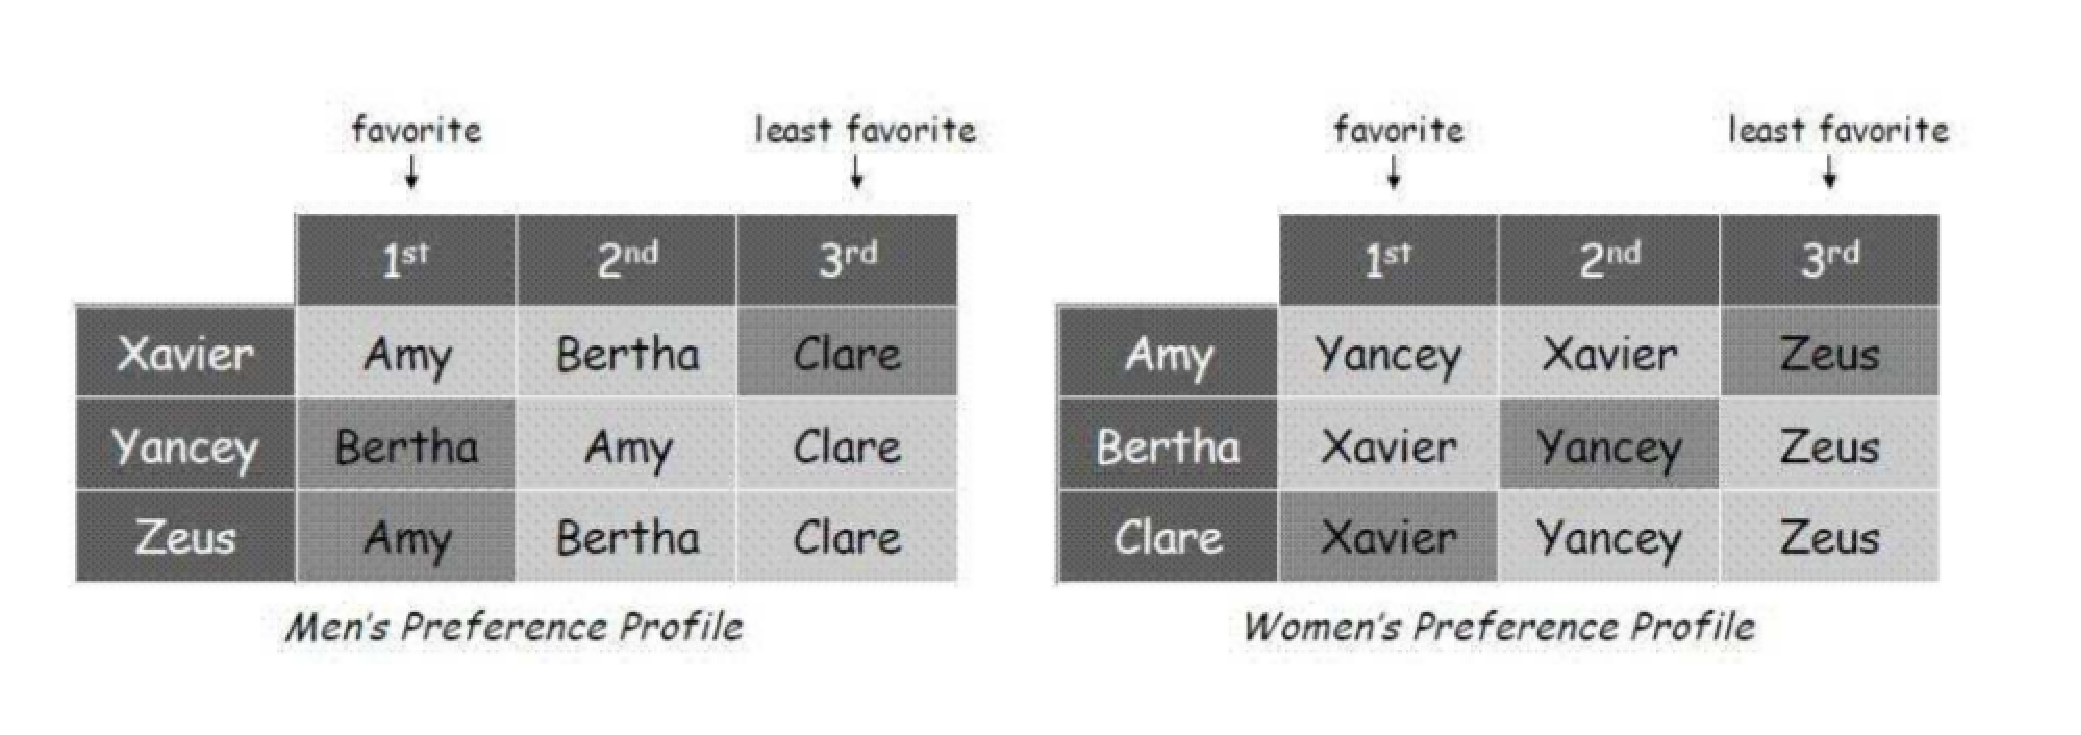
\includegraphics[width=15cm]{picture.eps}
	\caption{Preference Table}
\end{figure}

%插入表格
\begin{tabular}{|c|c|c|c|}\hline
{\bf METHODS}{\bf \cellcolor[gray]{.7}  No.}   & item1  & item2 & item3 \\\hline
{\emph MergeSort} & *    & *   & *  \\\hline
{\emph QuickSort} & *    & *   & *  \\\hline
{\emph M\_QuickSort} & * & *   & *  \\\hline
{\emph MergeSort\_Stack} & *   & *   & *  \\\hline
{\emph QuickSort\_Stack} & *    & *   & *  \\\hline
{\emph M\_QuickSort\_Stack} & *  & *   & *  \\\hline
\end{tabular}\\[5mm]

\end{CJK}
\end{document}
